\section{Procesja do Bożego Grobu}

\begin{itemize}
	\item \tt1 i \tt2 wychodzą z kadzielnicami, \oo~ - z ombrelino, \ding{63}
	      staje z krzyżem procesyjnym u wejścia do prezbiterium
	\item ministranci zapalają swoje świece
	\item \aa1 przynosi na ołtarz monstrancje i przejrzysty welon do niej
	\item \ii~ wraz z \cc1 i \cc2 udaje się do stopni ołtarza i sam wchodzi na
	      górę
	\item po wystawieniu Najświętszego Sakramentu \ii~ schodzi po stopniach,
	      zasypuje kadzidło i okadza N. S.
	\item po okadzeniu \cc2 nakłada \ii~ welon naramienny i wraca na miejsce
	\item \aa1 i \aa2 z akolitkami (wziętymi z kredensji) dołączają do \ding{63}
	\item \cc1 i \cc2 biorą kołatki
	\item gdy \ii~ bierze monstrancję, formuje się procesja w kolejności:

	      \begin{enumerate}\centering
		      \item[] (stopnie ołtarza)
		      \item[] \cc2~~~\ii~~~~\oo~~~~\cc1
		      \item[] \tt1~~~\tt2
		      \item[] chór ze świeczkami (parami)
		      \item[] \aa2~~~\ding{63}~~~\aa1
	      \end{enumerate}

	      \newpage

	      \begin{figure}[h]
		      \centering
		      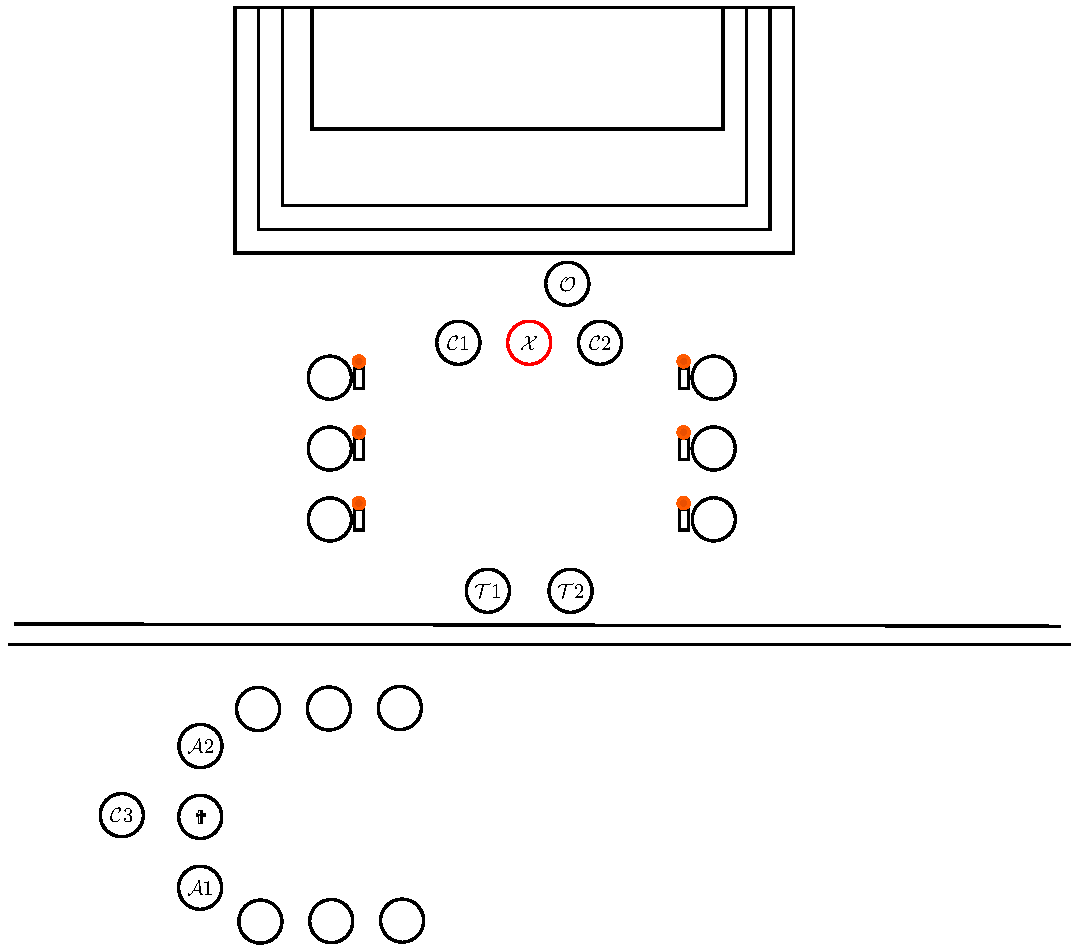
\includegraphics[scale=0.6]{Piatek/Procesja1.pdf}
	      \end{figure}

	\item po dokonaniu wystawienia w Bożym Grobie następuje zasypanie i
	      okadzenie oraz krótka adoracja

	      \begin{figure}[h]
		      \centering
		      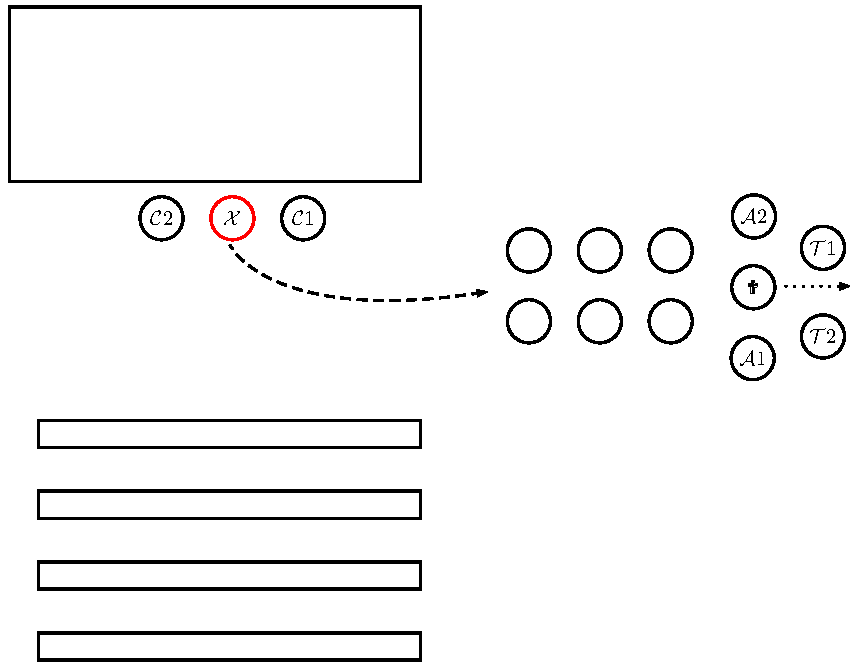
\includegraphics[scale=0.7]{Piatek/Procesja2.pdf}
	      \end{figure}

	\item procesja udaje się do zakrysti
\end{itemize}

